\documentclass[tikz,border=10pt]{beamer}
\setbeamertemplate{mini frames}{}
\usepackage{xcolor,colortbl}
\usepackage{amsthm}
\usepackage{amsmath}
\usepackage{amssymb}
\usepackage{array}
\usepackage{hyperref}
\usepackage[magyar]{babel}
\usepackage{t1enc}
\usetheme{Warsaw}
\usecolortheme{rose}
\frenchspacing
\usepackage{xkeyval}
\usepackage{wrapfig}
\usepackage{animate}
\usepackage{grffile}
\usepackage{media9}
\usepackage{multimedia}
\usepackage{graphicx}
\usepackage[bigfiles]{pdfbase}
\usepackage{tikz}
\usepackage{pifont}
\usetikzlibrary{matrix}
\usepackage{tabularx}

\newcolumntype{P}[1]{>{\centering\arraybackslash}p{#1}}
\newcolumntype{M}[1]{>{\centering\arraybackslash}m{#1}}


\beamerdefaultoverlayspecification{<+->}

\title{Videókártyák}
\author{Kórád György, \\ Buha Milán}
\date{2022}

\begin{document}

\tikzset{ 
    table/.style={
        matrix of nodes,
        row sep=-\pgflinewidth,
        column sep=-\pgflinewidth,
        nodes={
            rectangle,
            draw=black,
            align=center
        },
        minimum height=0.5em,
        text depth=0.5ex,
        nodes in empty cells,
%%
        every even row/.style={
            nodes={fill=gray!20}
        },
        column 1/.style={
            nodes={text width=6.2em,font=\bfseries}
        },
        row 1/.style={
            nodes={
                fill=gray,
                text=white,
                font=\bfseries,
            	text height=1.0em,
            	text depth=1.1em
            }
        }
    }
}

\frame{\titlepage}
\frame{\tableofcontents}

\section{Bevezetés}
\begin{frame}
\frametitle{Bevezetés}
\framesubtitle{Mi az a videókártya?}
Feladata, hogy a számítógép által küldött képi információkat feldolgozza, és egy megjelenítő egység számára értelmezhető analóg jelekké alakítsa. Ez az egység monitor, TV vagy kivetítő is lehet. A grafikus kártya és a megjelenítő különböző grafikus szabványok szerint kommunikálhat egymással. A videókártya a kivitelezés alapján lehet alaplapra integrált vagy bővítőkártya.
\end{frame}

\subsection{Története}
\begin{frame}
\frametitle{Bevezetés}
\framesubtitle{Története}
\transwipe[direction=90]
\begin{wrapfigure}{r}{0.3\textwidth}
    \centering
    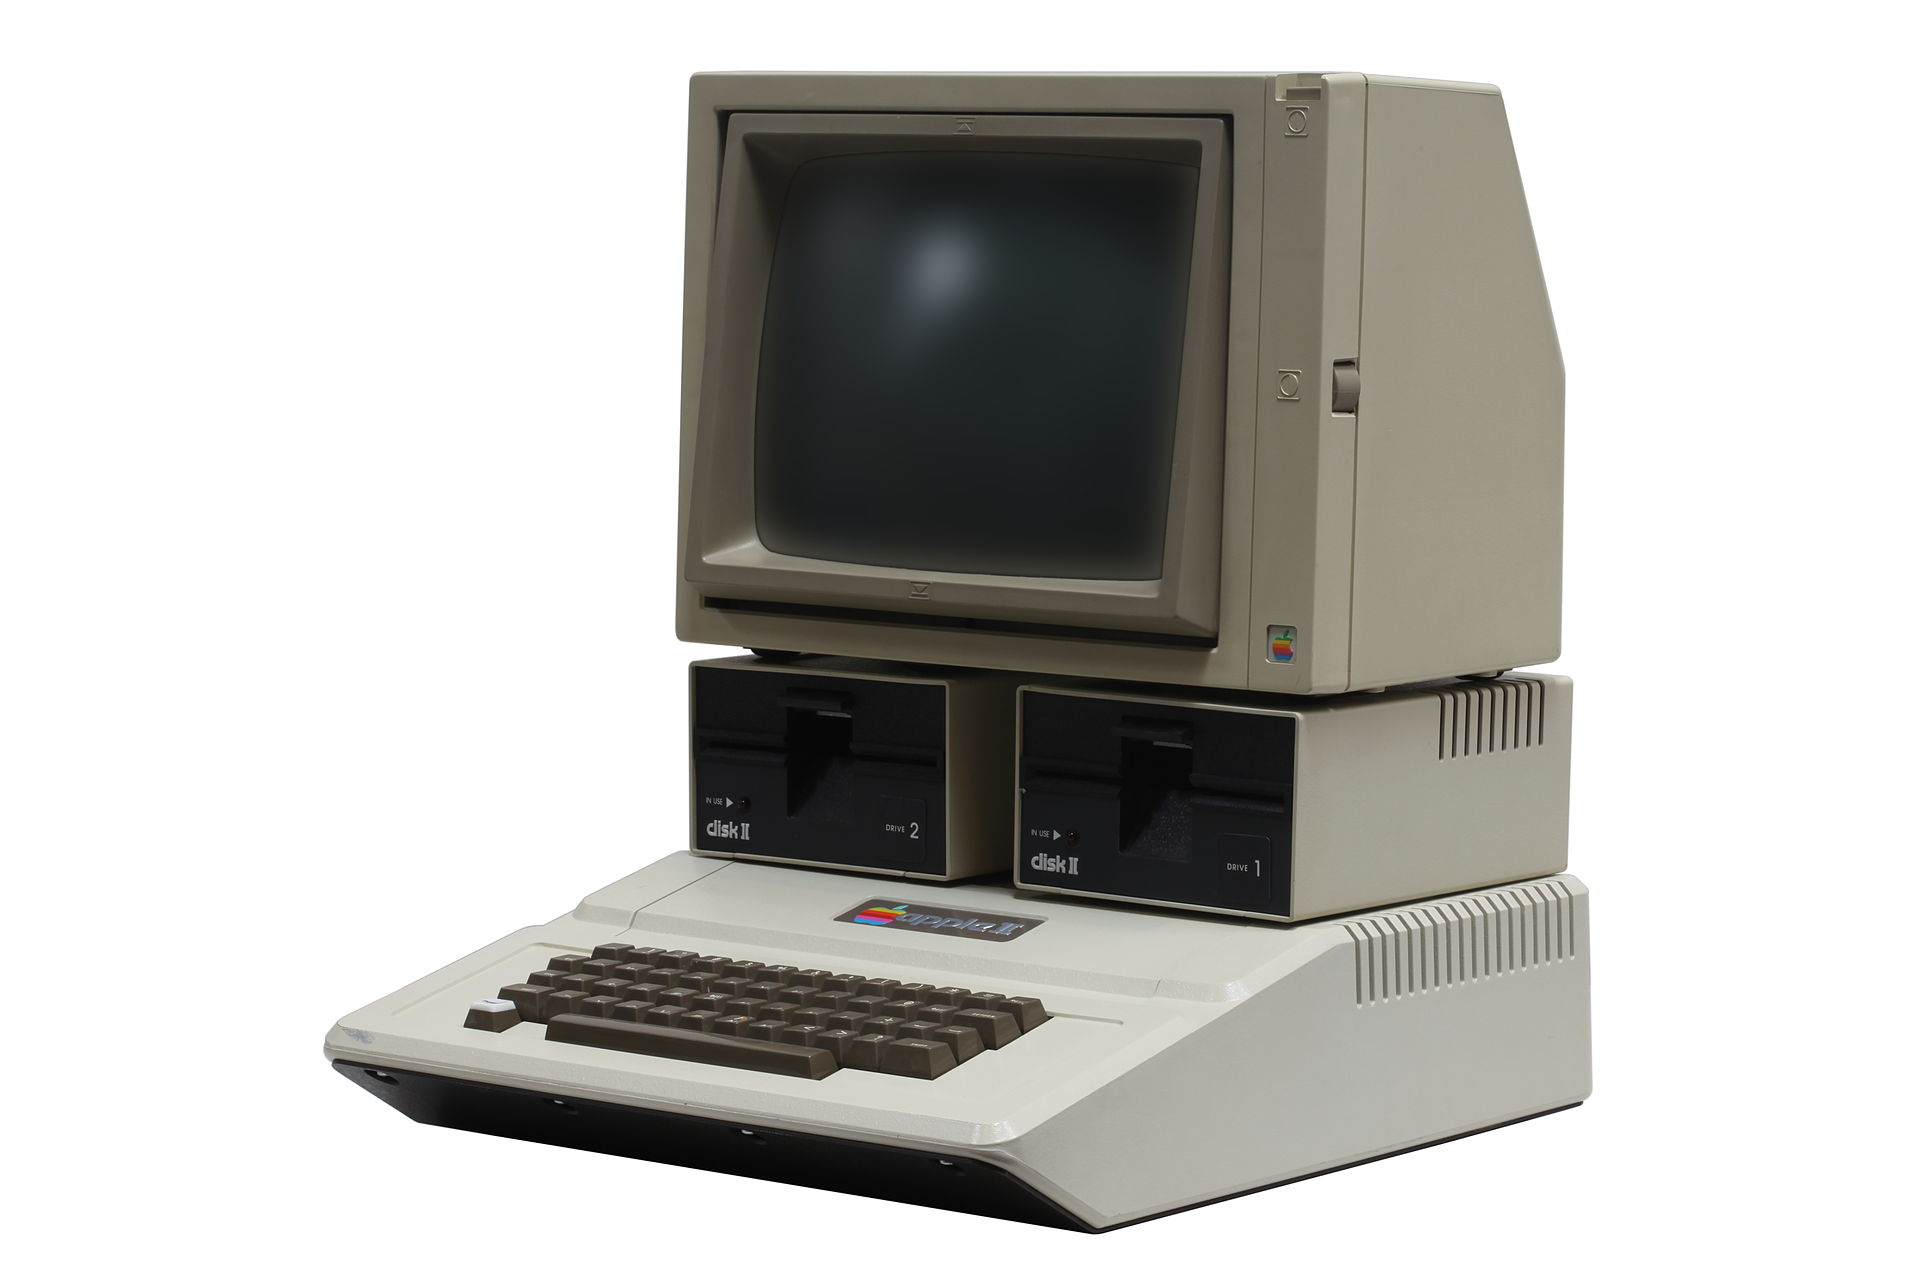
\includegraphics[scale=.05]{Media/Apple2.jpg}
    \caption{Apple II}
\end{wrapfigure}

Sorozatgyártásban a videókártya elvét elsőként 1977-ben az Apple II mikroszámítógép konstrukciójánál alkalmazták, melynek alaplapjára integrált képmegjelenítési lehetőségeit bővítőkártyák által lehetett kiegészíteni.
\end{frame}

\begin{frame}
\frametitle{Bevezetés}
\framesubtitle{Története}
\transwipe[direction=90]
\begin{wrapfigure}{r}{0.3\textwidth}
    \centering
    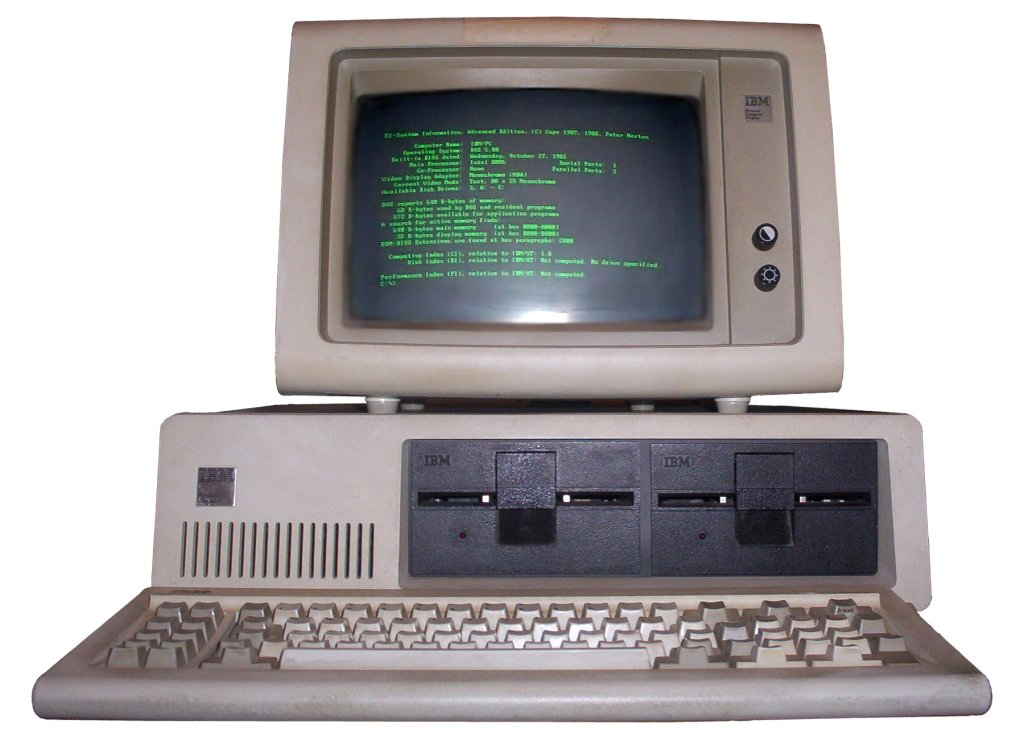
\includegraphics[scale=.09]{Media/ibmpc.jpg}
    \caption{IBM PC}
\end{wrapfigure}

Az első IBM PC 1981-ben kiadott típusában alkalmazott MDA (Monochrome Display Adapter) videókártya csupán az egyszínű, 80x25 karakteres megjelenítést tette lehetővé. Ezt követően az IBM CGA (Color Graphics Adapter) és a Hercules 1982-ben megjelent HGC (Hercules Graphics Card) videókártyái már a színes szövegkarakterek megjelenítését is támogatták.

\footnotetext[1]{\tiny https://hu.wikipedia.org/wiki/Videókártya}
\end{frame}

\subsection{GPU-k fejlődése}
\begin{frame}
\frametitle{GPU-k fejlődése}
\transwipe[direction=90]
\begin{columns}[onlytextwidth]
\begin{column}{0.5\textwidth}
\centering

\begin{figure}
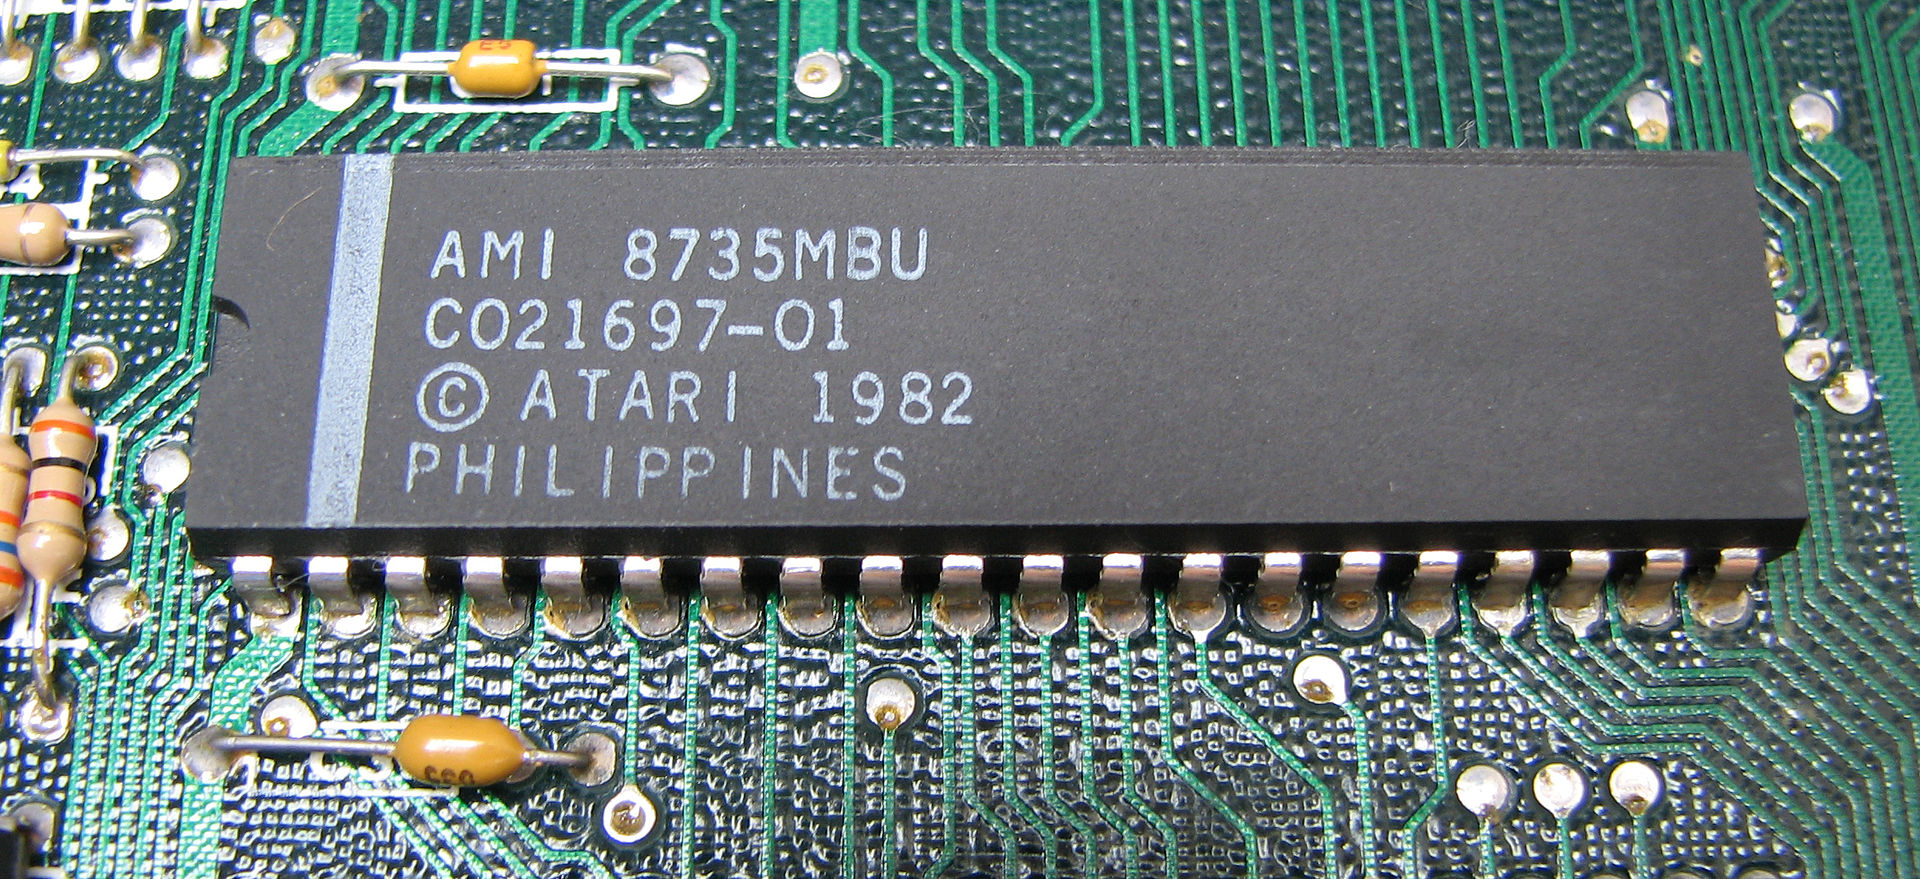
\includegraphics[scale=.14]{media/antic}
\caption{Atari ANTIC 1970-es évek}
\end{figure}

\begin{figure}
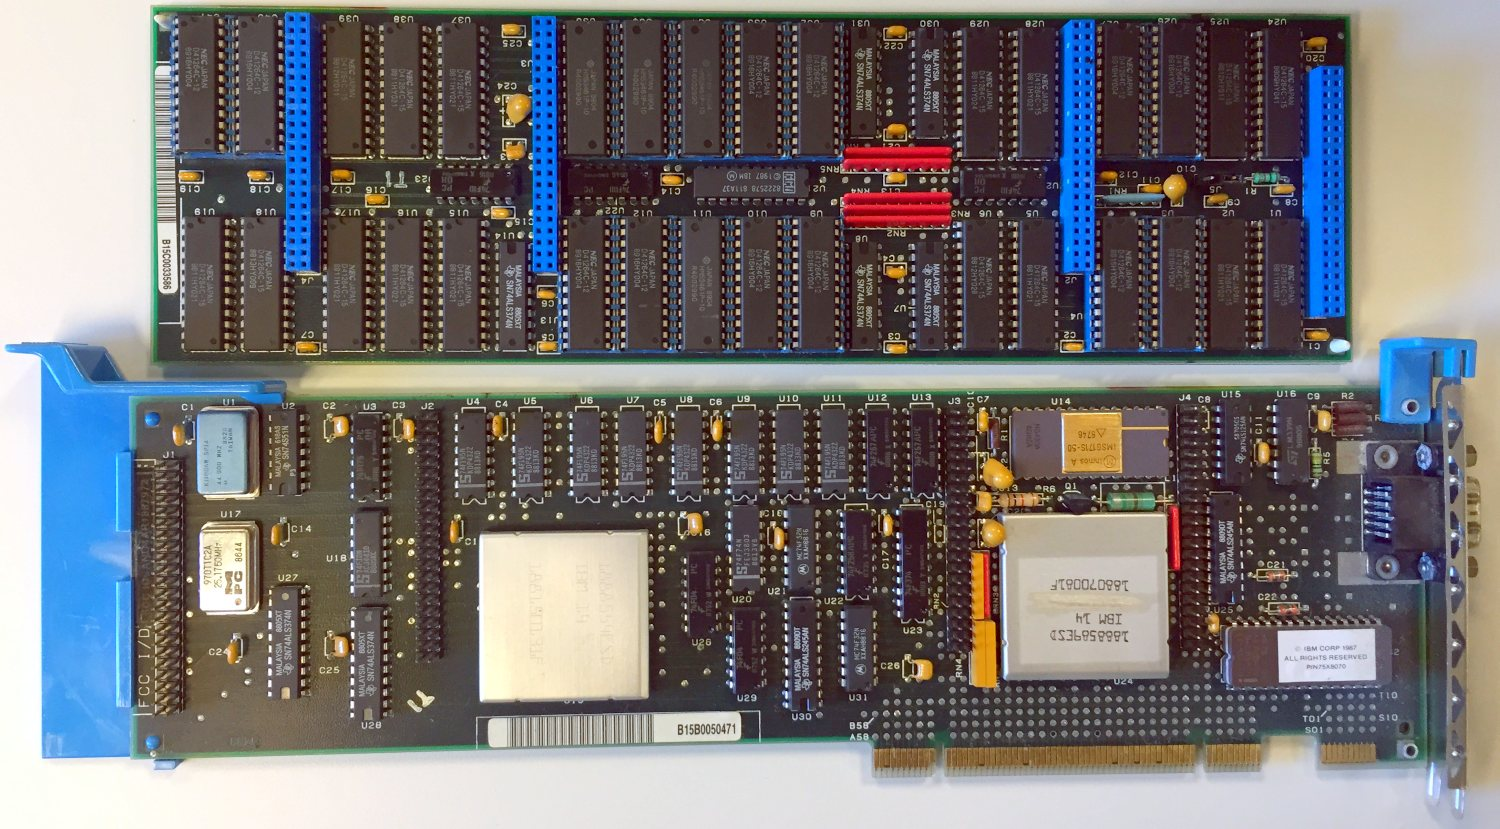
\includegraphics[scale=.0715]{media/ibm}
\caption{IBM 8514 1980-as évek}
\end{figure}

\end{column}
\begin{column}{0.5\textwidth}
\centering

\begin{figure}
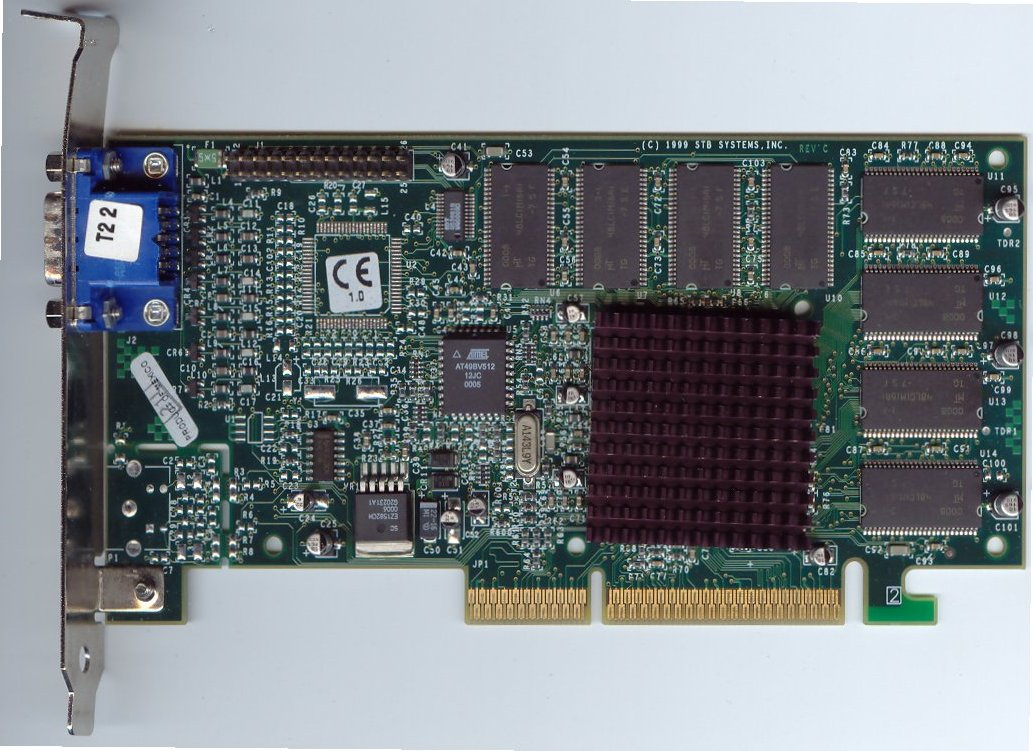
\includegraphics[scale=.15]{media/Voodoo3.jpg}
\caption{Voodoo3 1990-es évek}
\end{figure}

\begin{figure}
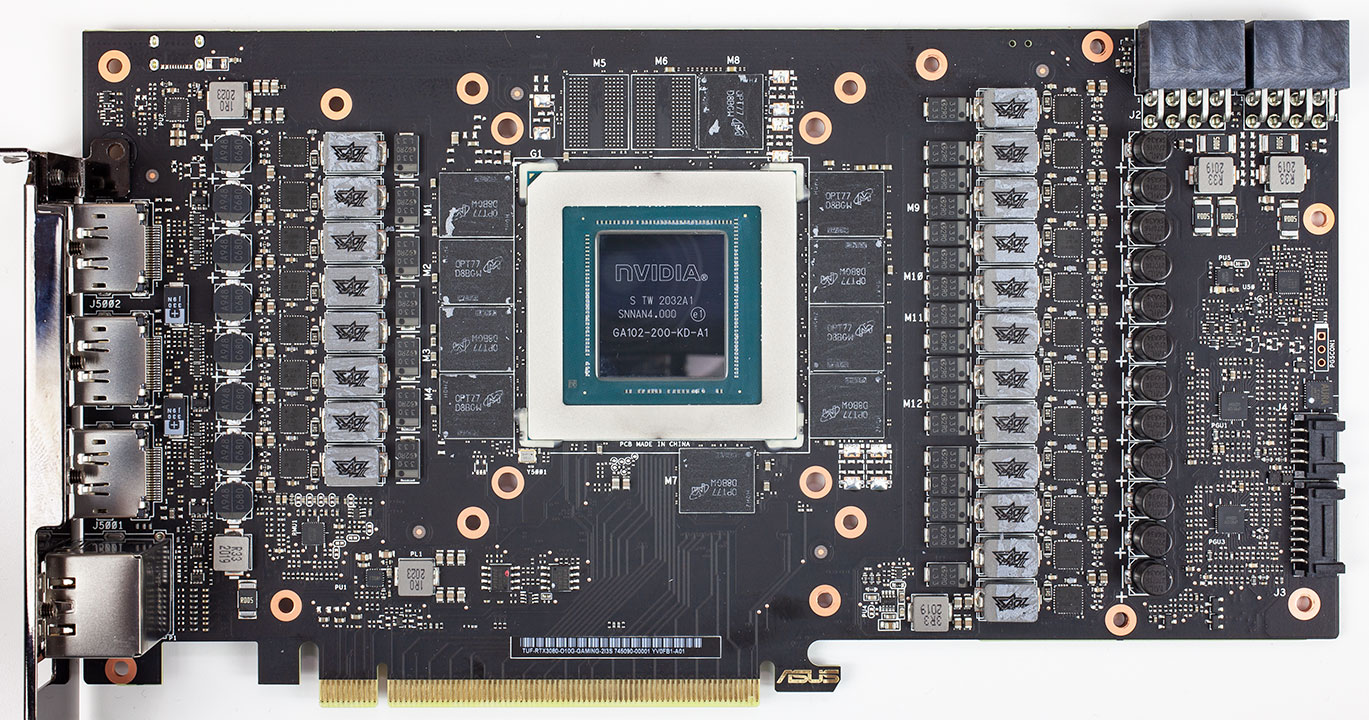
\includegraphics[scale=.078]{media/3080.jpg}
\caption{Nvidia RTX 3090 napjainkban}
\end{figure}

\end{column}
\end{columns}
\end{frame}

\section{Felépítés}
\begin{frame}
\frametitle{Vidókártyák felépítése}
\transwipe[direction=180]
\begin{figure}
\centering
\framebox{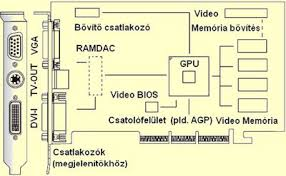
\includegraphics[scale=.5]{media/build.jpg}}
\caption{Egyszerűsített tervrajz}
\end{figure}

\end{frame}

\subsection{GPU}
\begin{frame}
\frametitle{Vidókártyák felépítése}
\framesubtitle{GPU [Graphics Processing Unit]}
\transwipe[direction=90]
A videókártya legfontosabb része, egy speciális processzor, ami grafikai műveleteket old meg 2 illetve 3 dimenzióban.\\
Feladata a grafikákat létrehozó feladatok átvétele a CPU-tól, így a processzornak nem kell grafikai számításokat végeznie, ezzel felgyorsítva a működését.\\
Hasonlóan mint a CPU a GPU is rendelkezik működési órajellel, ami a sebességét határozza meg.
\end{frame}

\subsection{Video memória}
\begin{frame}
\transwipe[direction=90]
\frametitle{Vidókártyák felépítése}
\framesubtitle{Video memória}
A video memória feladata a monitoron megjelenítendő képek tárolása. A Frame-buffer a
memóriaterület azon része (akkora képpontmátrix, amekkora a képernyő felbontás),
amelybe a kiszámolt és véglegesített képpontok kerülnek. Innen jut az elkészült kép a
\textbf{RAMDAC}-on keresztül a monitorra.
\end{frame}

\subsection{Csatlakozók}
\begin{frame}
\frametitle{Vidókártyák felépítése}
\framesubtitle{Csatlakozók}
\transwipe[direction=90]
\begin{columns}[onlytextwidth]
\begin{column}{0.3\textwidth}
\begin{figure}
\centering
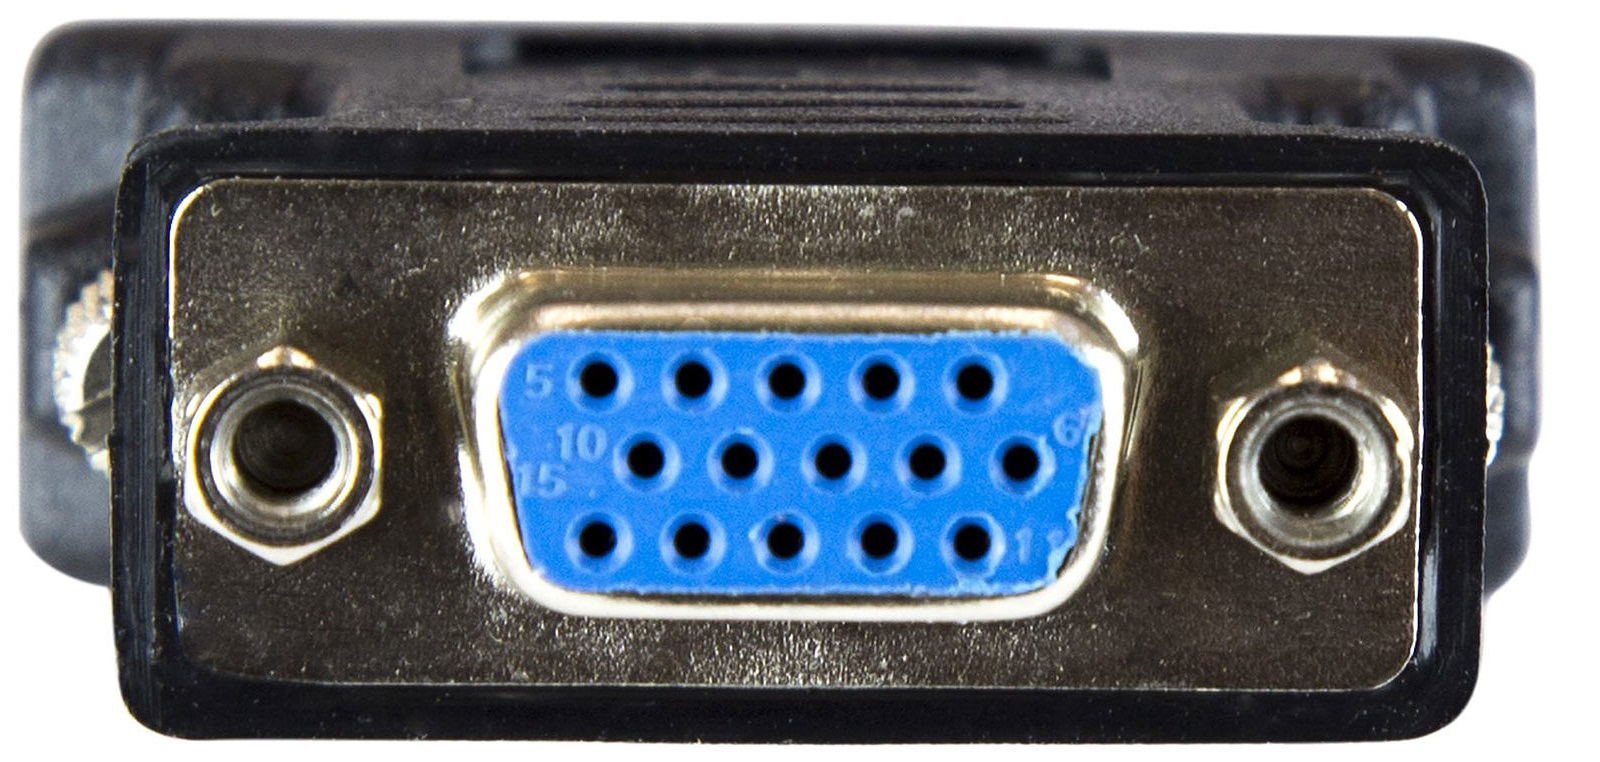
\includegraphics[scale=.075]{media/vga.jpg}
\caption{VGA}
\end{figure}
\end{column}

\begin{column}{0.3\textwidth}
\begin{figure}
\centering
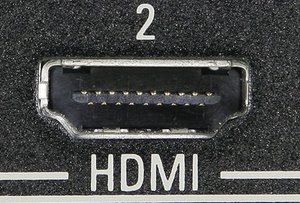
\includegraphics[scale=.25]{media/hdmi.jpg}
\caption{HDMI}
\end{figure}
\end{column}

\begin{column}{0.3\textwidth}
\begin{figure}
\centering
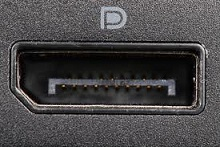
\includegraphics[scale=.45]{media/dp.jpeg}
\caption{DisplayPort}
\end{figure}
\end{column}

\bigskip
\end{columns}
A
videokártya ezeken keresztül biztosítja a csatlakoztatott monitor teljes működtetésével a
képernyőn történő megjelenítést.
\end{frame}

\subsection{Előnyök-Hátrányok}
\begin{frame}[fragile]
\hspace*{-30px}
\begin{tikzpicture}[ampersand replacement=\&]

\matrix (first) [table,text width=3em]
{
\& HDMI 1.2 \& HDMI 2.0 \& HDMI 2.1 \& DP 1.2 \& DP 1.3 \& DP 1.4 \& DP 2.0\\
1080p@120Hz   \& \ding{51} \& \ding{51} \& \ding{51} \& \ding{51} \& \ding{51} \& \ding{51} \& \ding{51}\\
1440p@30Hz   \& \ding{51} \& \ding{51} \& \ding{51} \& \ding{51} \& \ding{51} \& \ding{51} \& \ding{51}\\
1440p@60Hz   \& \ding{51} \& \ding{51} \& \ding{51} \& \ding{51} \& \ding{51} \& \ding{51} \& \ding{51}\\
1440p@120Hz   \& \ding{53} \& \ding{51} \& \ding{51} \& \ding{51} \& \ding{51} \& \ding{51} \& \ding{51}\\
4k@30Hz   \& \ding{51} \& \ding{51} \& \ding{51} \& \ding{51} \& \ding{51} \& \ding{51} \& \ding{51}\\
4k@60Hz   \& \ding{53} \& \ding{51} \& \ding{51} \& \ding{51} \& \ding{51} \& \ding{51} \& \ding{51}\\
4k@120Hz   \& \ding{53} \& \ding{53} \& \ding{51} \& \ding{53} \& \ding{51} \& \ding{51} \& \ding{51}\\
8k@30Hz   \& \ding{53} \& \ding{53} \& \ding{51} \& \ding{53} \& \ding{51} \& \ding{51} \& \ding{51}\\
8k@60Hz   \& \ding{53} \& \ding{53} \& \ding{51} \& \ding{53} \& \ding{53} \& \ding{51} \& \ding{51}\\
8k@120Hz   \& \ding{53} \& \ding{53} \& \ding{51} \& \ding{53} \& \ding{53} \& \ding{53} \& \ding{51}\\
};

\end{tikzpicture}
\end{frame}

\section{Beépítés}
\begin{frame}
\frametitle{Beépítés a számítógépbe}
\transwipe[direction=90]
A mai videókártyákat a számítógép \textbf{PCI-e} (Peripheral Component Interconnect) csatlakozójába illesztve, és ha szükséges táp ellátást biztosítva tudjuk használni a gyártó által biztosított illesztőprogrammal.

\begin{figure}
\centering
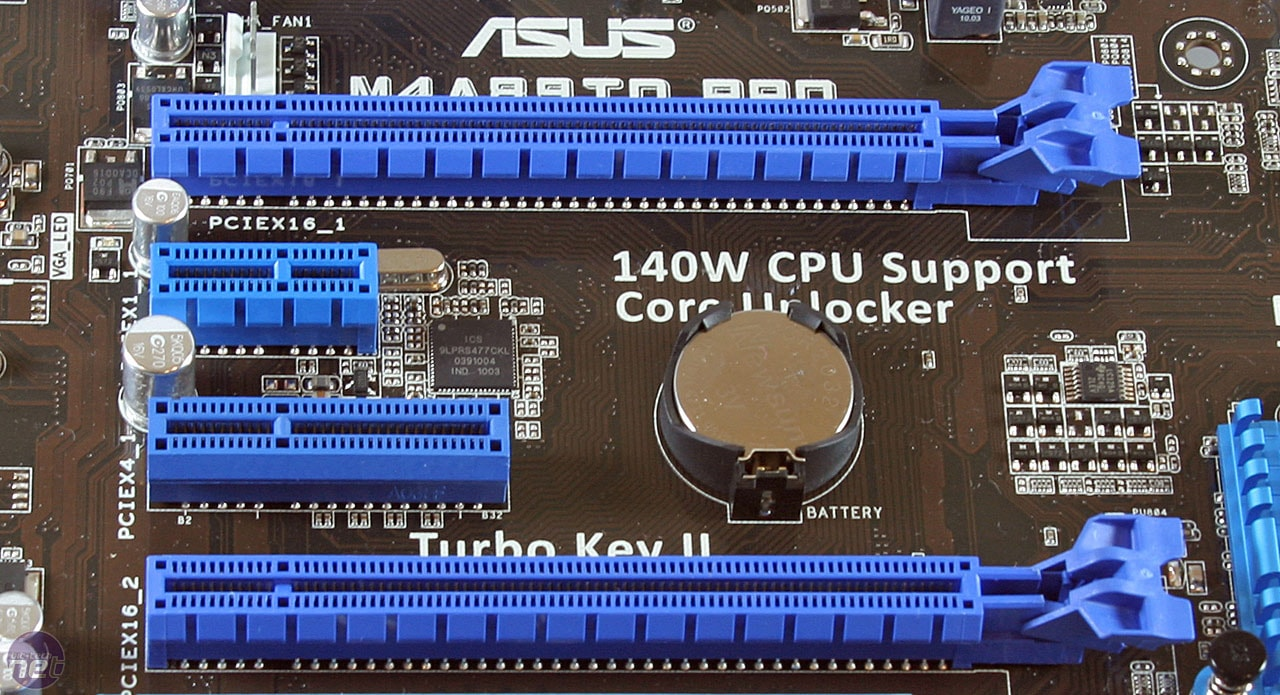
\includegraphics[scale=.09]{media/pci.jpg}
\caption{PCI-e csatlakozók}
\end{figure}
\end{frame}

\section{Ray tracing}
\begin{frame}
\frametitle{Ray tracing}

\transwipe[direction=180]

A ray tracing egy technológia, mely a megfigyelő helyzetén alapuló valós idejű sugárkövetés módszerét használja a kép kiszámításához. Ennek köszönhetően rendkívül hű szimulációt valósít meg.
\\
\textbf{Ray tracing videókártyák:}
\begin{columns}[onlytextwidth]
\begin{column}{.5\textwidth}

\begin{itemize}
\item<1-> Nvidia \pause
\begin{itemize}
\item RTX 20 series 
\item RTX 30 series 
\item RTX 40 series 
\end{itemize}
\end{itemize}
\end{column}

\begin{column}{.5\textwidth}
\begin{itemize}
\item<2-> AMD \pause
\begin{itemize}
\item Radeon RX 6600 XT 
\item Radeon RX 6700 XT 
\item Radeon RX 6800 XT 
\end{itemize}

\end{itemize}

\end{column}
\end{columns}
\end{frame}

\section{Számítási teljesítmény}
\begin{frame}

\arrayrulecolor{blue}

\setlength{\arrayrulewidth}{0.5mm}
\setlength{\tabcolsep}{18pt}
\renewcommand{\arraystretch}{1.3}
\centering
\begin{tabular}{|P{3cm}|P{3cm}|}
\hline
\multicolumn{2}{|c|}{Számítási teljesítmény} \\
\hline
ÉV & TFLOPS\\
\hline
2008 & 0\hspace{1pt}.2\\
2010 & 0\hspace{1pt}.5\\
2012 & 1\hspace{1pt}.2\\
2014 & 2\hspace{1pt}.8\\
2016 & 5\hspace{1pt}.5\\
2018 & 1\hspace{1pt}4.2\\
2020 & 3\hspace{2pt}4.1\\
2022 & 9\hspace{2pt}5.4\\
\hline
\end{tabular}
\end{frame}

\section{RTX Videó}
\begin{frame}
\begin{center}
\begin{figure}
\movie[externalviewer]
  {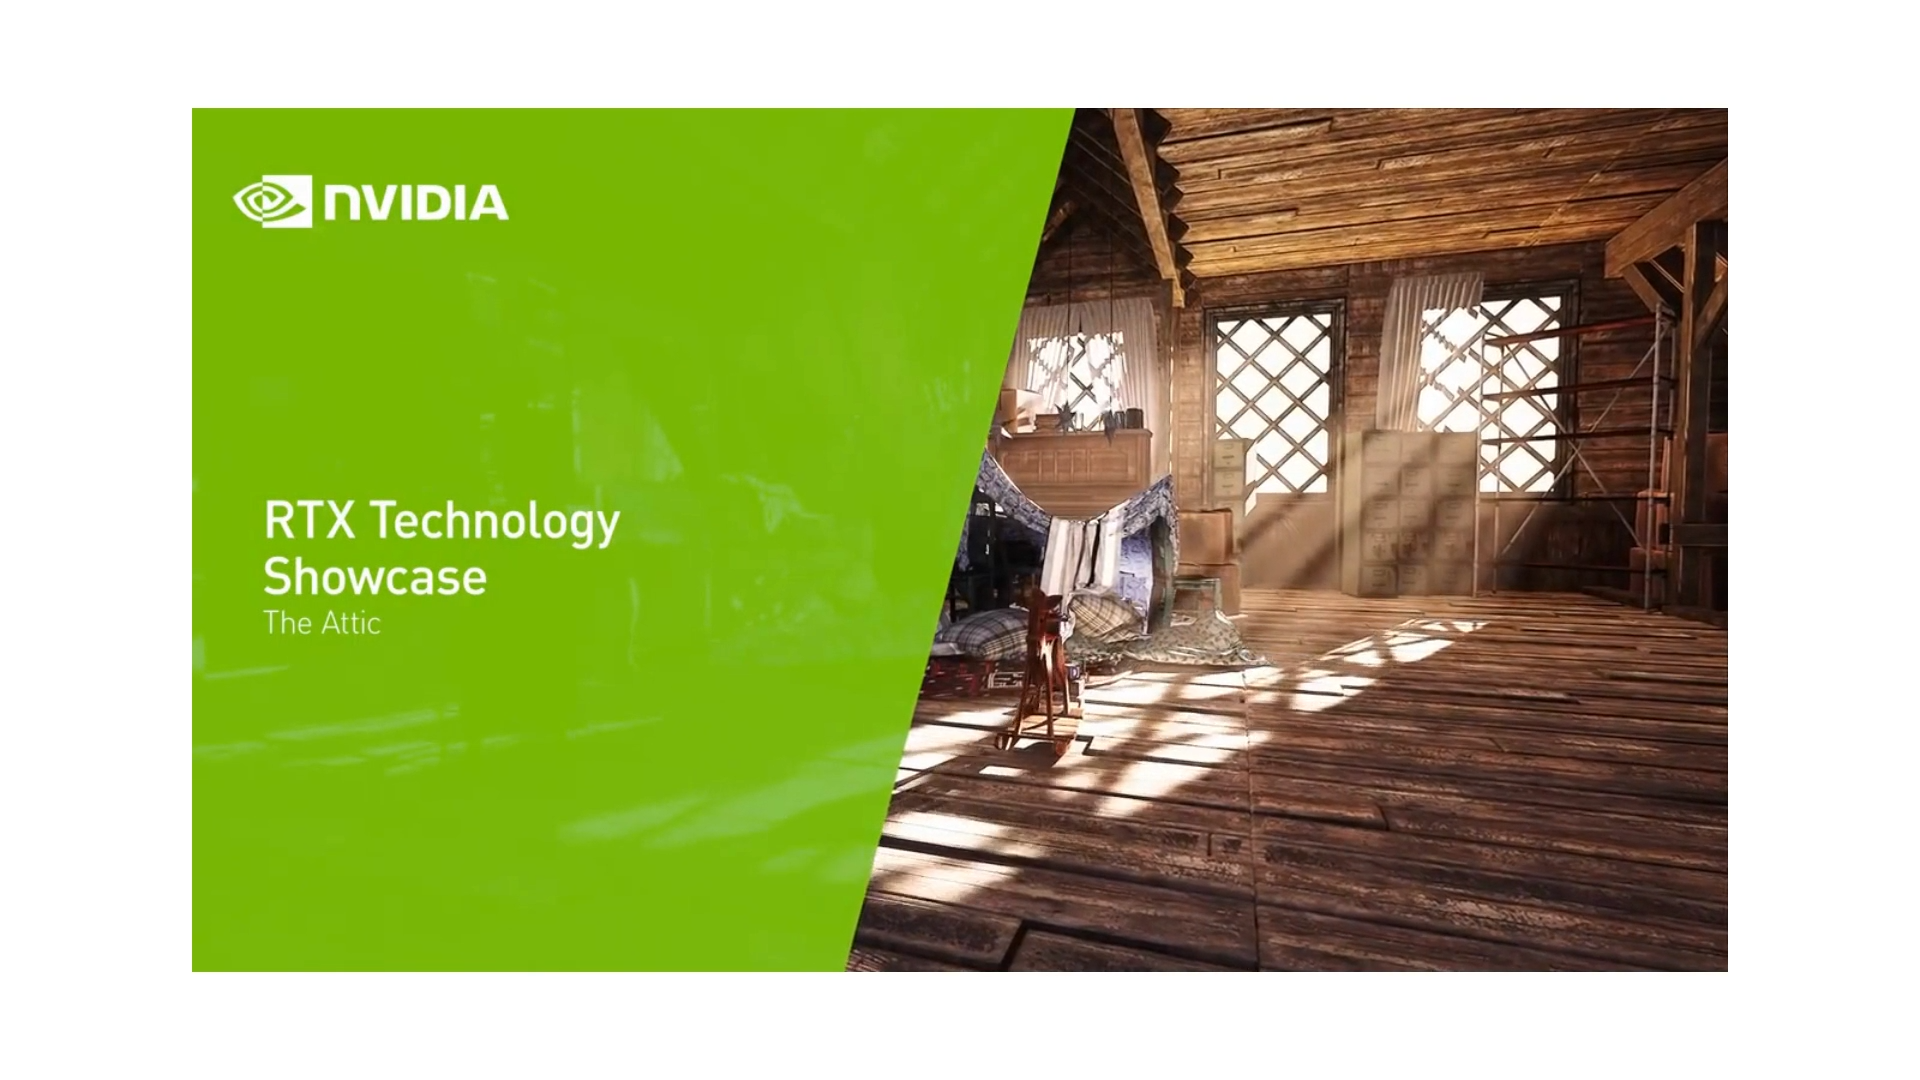
\includegraphics[width=1.0\textwidth]{media/image.png}}{media/RTX.mp4}
\caption{A videó lejátszásához kattintson a képre!}
\end{figure}
\end{center}
\end{frame}

\begin{frame}
\begin{center}
\begin{huge}
Köszönjük a figyelmet!
\end{huge}
\end{center}
\end{frame}

\end{document}
